% This is the central and most important section of the report. Its objective must
% be to show, with linearity and clarity, the steps that have led to the
% definition of a decision model. The description of the working hypotheses,
% confirmed or denied, can be found in this section together with the description
% of the subsequent refining processes of the models. Comparisons between
% different models (e.g. heuristics vs. optimal models) in terms of quality of
% solutions, their explainability and execution times are welcome.

% Do not attempt to describe all the code in the system, and do not include large
% pieces of code in this section, use pseudo-code where necessary. Complete source
% code should be provided separately (in Appendixes, as separated material or as a
% link to an on-line repo). Instead pick out and describe just the pieces of code
% which, for example:

% \begin{itemize}
%     \item are especially critical to the operation of the system;
%     \item you feel might be of particular interest to the reader for some reason;
%     \item  illustrate a non-standard or innovative way of implementing an algorithm, data
%           structure, etc..
% \end{itemize}

% You should also mention any unforeseen problems you encountered when implementing the
% system and how and to what extent you overcame them. Common problems are:
% difficulties involving existing software.

Inizialmente sono state valutate le performance a
partire dalle sole features non testuali così da stabilire un punto di
partenza per la successiva analisi di quelle testuali.

È stato utilizzato un semplice modello composto da due layer Densi entrambi
seguiti da un layer di Dropout con un layer Denso finale con funzione d'attivazione lineare.
Questo modello verrà in seguito ampliato per fare uso delle feature
testuali a seconda dei vari approcci.
La figura \ref{fig:modeltemplate} ne mostra un template.

\begin{figure}[h!]
	\centering
	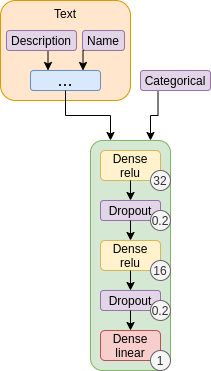
\includegraphics[
		height=6cm,
		keepaspectratio,
	]{modelTemplate.png}
	\caption{Template del modello con numero di neuroni e rate di dropout finali cerchiati}
	\label{fig:modeltemplate}
\end{figure}

% todo: mettere le performance nella sezione dopo
% todo: immagine del modello

% parlare di quanto tempo richiedono le 10 epoche.
% del numero dei parametri del modello.
% di quanti neuroni hanno i layers e perchè (magari fare una prova con vari
% valori bassi e aumentarli senza esagerare fino a raggiungere le performance sopra)
% parlare di qualche altro parametro? di training del modello?

\subsection{Rappresentazione del Testo}
% todo parlare della dimensionalità. di cosa è un dizionario

Sono stati valutati diversi approcci per il trattamento del testo partendo da
modelli semplici come \textit{Bag of Word} fino ai più recenti ed efficaci come
\textit{BERT}, passando per i \textit{Word Embedding}.

\subsubsection{Bag of Word}
% todo: dire qualcosa della dimensionalità di bow e tf idf?
Il modello bag-of-words permette di rappresentare il testo tramite un vettore
per ogni documento contenente il numero di occorrenze di ciascuna parola del
vocabolario nel documento; questi vettori hanno cardinalità pari alla dimensione
del vocabolario e assegnando 0 in caso di parole dal documento assenti sono
generalmente sparsi.

Regole grammaticali e ordine delle parole non sono rappresentabili
tramite questa tecnica \cite{manning_raghavan_schutze_2008}.

Ritornando al modello, per quanto riguarda Bag of Words i vettori delle feature
testuali sono forniti in input direttamente al primo layer denso allo stesso
modo delle variabili non testuali.

\subsubsection{Tf-Idf}\label{section-tfidf} Tf-Idf (Term frequency-Inverse
document frequency) \cite{manning_raghavan_schutze_2008} è una misura
dell'importanza di una parola rispetto al documento che la contiene in rapporto
all'importanza della stessa nell'intera collezione di documenti; segue la
definizione.% (corpus). ?
% todo: va bene parlare di documenti? vogliamo addattare più al nostro dataset?

\begin{equation}
	\label{eq:tf-idf}
	Tf\mbox{-}Idf_{t,d}
	=
	tf_{t,d} \cdot idf_t
	=
	\frac{n_{t,d}}{|d|} \cdot \log \frac{|D|}{|\{d: t \in d\}|}
\end{equation}

Dove $t$ indica il termine, $d$ il documento, $n_{t,d}$ la frequenza assoluta di
t in d, $D$ l'insieme dei documenti.

Per Tf-Idf come approccio di rappresentazione del testo si vuole indendere un
approccio simile a Bag of Word i cui vettori, anzichè contenere il
numero di occorrenze contengono il valore Tf-Idf (\ref{eq:tf-idf}) della parola.

All'interno del modello è stato utilizzato allo stesso modo di Bag
of Words.

\subsubsection{Word Embedding}

I cosiddetti \textit{word embedding} rappresentano parole per mezzo di vettori
densi di lunghezza fissa \cite{almeida2019word}, contrapponendosi a  \textit{Bag
	of words}.

Inoltre questi vettori sono in grado di apprendere relazioni semantiche e
sintattiche tra le parole \cite{mikolov2013efficient}.

% word embedding di keras
\subsubsection{Keras Embedding Layer}

Keras fornisce un implementazione di embedding sotto forma di layer neurale e
ne rende quindi possibile l'addestramento insieme a layer restanti.
% % todo dire dopo questa cosa con glove
% Offre inoltre la possibilità di fissare il valore dei pesi semplificando
% l'integrazione con modelli pre-allenati.
\\
Ritornando al modello, il testo in input è stato codificato in forma di
vettori di interi, tramite la classe \textit{tf.keras.preprocessing.\-text.Tokenizer}.

Tenendo come riferimento il template in figure
\ref{fig:modeltemplate}, nella sezione che tratta il testo, precisamente in
sostituzione al box ``...'' sono stati aggiunti due layer embedding, uno per
\textit{Name} e uno per \textit{Item\_description}, seguiti da layer aggiuntivi
per sfruttare al meglio le informazioni degli embedding di cui verrà discusso in
seguito.

Infine l'output di questi layer aggiuntivi è stato assegnato come input al primo
layer denso come mostrato. La figura \ref{fig:kerasModel} ne mostra uno schema.

\begin{figure}[h!]
	\centering
	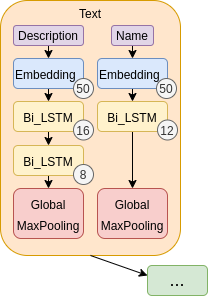
\includegraphics[
		height=5cm,
		keepaspectratio,
	]{kerasModel.png}
	\caption{Schema riassuntivo sulla gestione dei dati testuali, dove per Bi\_LSTM si intendono layer LSTM bidirezionali con dropout a 0.2 e i valori cerchiati identificano il numero di neuroni.}
	\label{fig:kerasModel}
\end{figure}

\subsubsection{GloVe}
GloVe (Global Vectors) è un modello non supervisionato in grado di costruire
word embedding a partire da statistiche globali (rispetto all'intero
corpus) di co-occorrenza delle varie parole \cite{pennington2014glove}. Sono
inoltre disponibili modelli GloVe pre-addestrati. Seguono quelli valutati nel
progetto.
\begin{itemize}
	\item GloVe6B (Wikipedia 2014 + Gigaword 5): con vettori di 50 dimensioni
	      allenati su 6 miliardi di parole, con un vocabolario di 400 mila
	      parole.
	\item GloVe840B (Common Crawl): con vettori di 300 dimensioni allenato su
	      840 miliardi di parole, con un vocabolario di 2.2 milioni parole.
\end{itemize}

Per quanto riguarda il modello è stata utilizzata la stessa architettura del
modello Keras assegnando i pesi preaddestrati e la corretta dimensionalità ai
layer Embedding e impostandoli come non-trainabili.

\subsubsection{Transformers}
% diremo che il trasform supera lstm. todo pro-cons lstm: tipo memoria,...
Il Transformer è un'architettura basata su di una struttura
\textit{encoder-decoder} che utilizza un meccanismo di
\textit{attention} per rappresentare i rapporti di dipendenza di input e output \cite{vaswani2017attention}.

% todo decidere se togliere l'anno

% BERT’s model architecture is a multi-layer bidirectional Transformer encoder
% based on the original implementation

Una dei più noti transformer è \textit{BERT}, \textit{Bidirectional Encoder
Representations from Transformers}), dove per bidirezionale si intende capace di
apprenderne relazioni sia con input precedenti che successivi, che si basa
esclusivamente su moduli encoder. Nasce per fornire un modello pre-allenato
adattabile a numerose applicazioni tramite \textit{fine-tuning}.
Tuttavia anche utilizzi \textit{feature-based} risultano efficaci
\cite{devlin2018bert}.

In questo progetto è stato utilizzato \textit{DistilBert}, una versione più leggera ottenuta
da BERT tramite \textit{Knowledge distillation} \cite{sanh2020distilbert}, con un approccio feature-based.

Ritornando al modello, occupa la stessa posizione dedicata agli embedding
(figura \ref{fig:kerasModel}) per entrambi i campi nome e descrizione.

\subsection{Training e valutazione}

\subsubsection{Dataset split}

Al fine di valutare i vari modelli più correttamente possibile il dataset è
stato suddiviso in \textit{training-set}, \textit{validation-set} e
\textit{test-set}.

\subsubsection{Valutazione dell'errore}
% loss e metriche

Per quanto riguarda le performance in termini di errore la funzione di
\textit{loss} utilizzata in fase di training è il \textit{Root Mean Squared
	Logaritmic Error (RMSLE)}; è inoltre la misura scelta dalla Kaggle challenge
per confrontare le performance dei vari partecipanti.

Seguono la definizione e alcune osservazioni su di RMSLE e MSLE.
\\
\textit{Root Mean Squared Logarithmic Error (MSLE)},
\begin{equation}
	RMSLE
	=
	\sqrt{
	\frac{1}{n}
	\sum_{i=1}^{n}
	( \log(y_i+1) - \log(\hat{y_i}+1) )^2
	}
	=
	\sqrt{
		\frac{1}{n}
		\sum_{i=1}^{n}
		\log^2(\frac{y_i+1}{\hat{y_i}+1})
	}
\end{equation}

Essendo calcolato a partire da un rapporto, riflette l'errore relativo e di
conseguenza risulta efficace laddove i valore assoluti presentano variazioni
considerevoli, come per i prezzi in esame.

% todo numero parametri

\subsubsection{Valutazione dei costi computazionali}

Per valutare dei costi computazionali sono stati annotati il numero dei
parametri allenabili e non dei vari modelli e il tempo richiesto dalle epoche di
allenamento sul trainset.

È stata utilizzata la piattaforma \textit{Google Colab} abilitando l'accelerazione hardware GPU.

\subsection{Parametri di training}
% todo sono risultati?

I parametri di training sono stati impostati in seguito a test sperimentali in
modo da minimizzare l'errore mantenendo accettabili i tempi di training richiesti.
